Un campo de fútbol rectangular tiene 64 metros de ancho y 100 metros de largo.
Un jugador corre en diagonal desde una esquina del campo hasta la esquina opuesta.

\textbf{¿Cuánto corrió el jugador?}\\
\textit{Redondea tu respuesta al metro más cercano.}


\begin{solutionbox}{13cm}
    Tratamos de determinar $x$ en la siguiente imagen:
    \begin{figure}[H]
        \centering
        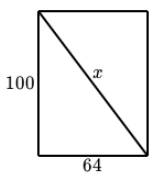
\includegraphics[width=0.2\linewidth]{../images/proverb_pitagoras_12.png}
        \caption{}
        \label{fig:proverb_pitagoras_12}
    \end{figure}
    Podemos usar el teorema de Pitágoras para obtener $x$.
    La ecuación del teorema de Pitágoras es:
    \[c^2=a^2+b^2\]
    donde $a$ y $b$ son las longitudes de los dos catetos del triángulo y $c$ es la longitud de la hipotenusa.
    En este caso, $a=64$, $b=100$ y $c=x$.
    \begin{align*}
        x^2 & =64^2+100^2    \\
        x^2 & = 14,096       \\
        x   & =\sqrt{14,096} \\
        x   & \sim 119
    \end{align*}
    El jugador corrió aproximadamente 119 metros.
\end{solutionbox}